%File: formatting-instruction.tex
\documentclass[letterpaper]{article}
\usepackage{aaai}
\usepackage{times}
\usepackage{helvet}
\usepackage{courier}
\usepackage{graphicx}
\frenchspacing
\setlength{\pdfpagewidth}{8.5in}
\setlength{\pdfpageheight}{11in}
\pdfinfo{
/Title (Insert Your Title Here)
/Author (Put All Your Authors Here, Separated by Commas)}
\setcounter{secnumdepth}{0}  
 \begin{document}
% The file aaai.sty is the style file for AAAI Press 
% proceedings, working notes, and technical reports.
%
\title{CS 4080-5080: Reinforcement Learning\\Homework Assignment One}
\author{University of Colorado Colorado Springs\\Jacob Quatkemeyer
}
\maketitle
\begin{abstract}
\begin{quote}
The paper acts as a write up to homework assignment one in the class CS 4080-5080: Reinforcement Learning. The idea was to implement a simple reinforcement learning agent, from scratch,  in a programming language of our choosing.This task had to be accomplished without using any reinforement learning modules or libraries.
\end{quote}
\end{abstract}

\section{Introduction}
\noindent Consider  the  simple  maze  we  have  been  talking  about  in  the  class  as  we  discuss  concepts  and algorithms in reinforcement learning.  It is a 5×5 grid, with a single start state and a single goal state as shown in Figure 1.  

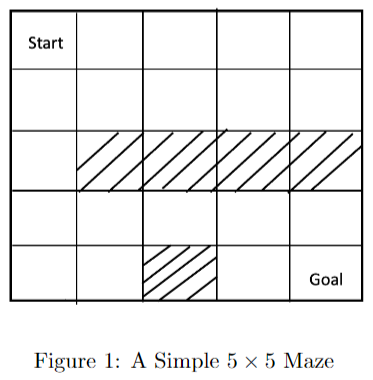
\includegraphics{figure_1}

There is a barrier to movement covering four states in the third row. There is also a barrier to movement in the middle of the fifth row.

The agent needs to learn a policy that will take it from the start state to the goal state efficiently.

\begin{enumerate}
\item How would you represent the various components that are required to program this reinforcement learning agent? Discuss each component and how you implement it. Explain how you model the barriers, and how you make sure the agent does not fall off the edges.
\item You would initialize with a random policy where every action that is possible in a state is equally probable. What does this policy look like?
\item Assume the agent uses a Monte Carlo method to learn an optimal policy starting with the equi-random policy. It involves improving the random policy slowly using a greedy approach and stopping when the policy does not improve any more. Write the algorithm in terms of pseudocode and briefly explain with reference to lines in the pseudocode.
\item Implement the algorithm using any programming language of choice. Run the algorithm several times. Does it produce the same policy every time? Show the policy  (policies) learned. Explain any differences if any. Change any relevant parameters and rerun a few times. Comment on how changes in parameter values changes learning.
\item Write a short paper giving details of what you have done, the results you have obtained, the problems you have faced, and how you have overcome the problems you have faced. Use the format you use for your semester project papers. The maximum number of pages is 4 for content, followed by an extra page for references, if necessary.
\item Extra credit may be given based on substantial additional work. For example, you can discuss and implement more than one Monte Carlo algorithm, based on limitations of the  (first) approach that you try. You may also discuss metrics to measure how the agent learns and performs after learning, implement such metrics. This part of the homework is intentionally left open-ended.
\end{enumerate}

\section{Question One}
\noindent The various components required to program this reinforcement learning agent include: 
\begin{itemize}
\item Policy
\item Q-Table
\item Return Table
\item Gamma Value
\item Epsilon Value / Epsilon Decay
\item Data Structure for First Visit MC
\end{itemize}

The policy is the agent's stategy, or each action that the agent should take at each state to maximize reward. In Python for instance, this can look like a dictionary whose keys are each of the available states, and whose values are the actions the agent should take at each state. In monte carlo learning, it is useful to initially instantiate this policy randomly, with each action randomly chosen from each states available actions. This initial random policy allows us to explore the environment, calculate the overall return of each state and action, find the average return, and update our Q-Table. With the updated Q-Table, we can edit our policy, and repeat the previous steps to further improve our policy. 

The Q-Table is simply a lookup table where we calculate the maximum expected future rewards for each action at each state. This is a very useful data structure as it includes the set of each available action for each state in the set each available state, allowing us to keep the agent within the bounds of the maze, and outside of the barriers. For instance, if the agent is at the starting state 'cell00', taking the actions 'Left' or 'Up' would take the agent outside of the maze. To solve this, we simply instantiate state 'cell00' with the only available actions being 'Right' and 'Down' i.e, we limit the action space. Each action is initially instantiated with a value of '0' as there is initially no information about the expected future rewards. Once these values are updated, it is simple to create a policy by simply looking immediately ahead at the next states in the Q-Table, and choosing the action that would maximize the greatest reward.

The Return Table is very similar to the Q-Table, and it is vital to updating the Q-Table with the maximum expected future rewards. The table holds the average of all of the cumulative

\section{References}
\smallskip \noindent \textit{Automated trading systems statistical and machine learning methods and hardware implementation: A survey Enterprise Information Systems}\\
B. Huang, Y. Huan, L.D. Xu, L. Zheng, Z. Zou 2019. \textit{Blackboard Systems.} 13 (1) (2019), pp. 132-144


\end{document}
